\documentclass[9pt]{beamer}

\beamertemplatenavigationsymbolsempty
\renewcommand\mathfamilydefault{cmr}

\usepackage{xcolor}
\usepackage{pajmath}
\usepackage{booktabs}
\usepackage{colortbl}
\usepackage{tikz}
\usetikzlibrary{calc}
\usetikzlibrary{intersections}
\usetikzlibrary{datavisualization}
\usetikzlibrary{datavisualization.formats.functions}

\title{Exam 2 Review}
\date{Spring 2021}

\begin{document}

\maketitle

\begin{frame}{Announcements}
\begin{itemize}
	\item Exam 2 will be ``take home'': 80 minutes from when you \textbf{begin} the exam.
	\item The exam \emph{must} be completed by 5pm Central time on Friday 3/26.
	\item I will have additional office hours on Thursday, 8:30--9:20am for last-minute questions.
\end{itemize}	
\end{frame}


\begin{frame}{RMSE of a linear model}

\begin{columns}
\begin{column}{0.4\textwidth}
	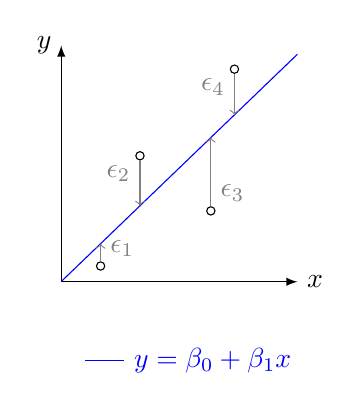
\begin{tikzpicture}
	\begin{scope}
		\draw [->,>=latex] (0,0) -- (3,0) node [right] {$x$};
		\draw [->,>=latex] (0,0) -- (0,3) node [left] {$y$};
		
		\draw [name path=model,domain=0:3,blue] plot (\x, {0.0027 + 0.9624*\x});
		
		\foreach \pt/\i in {(0.5,0.2)/1, (1.9,0.9)/3, (2.2,2.7)/4, (1.0,1.6)/2} {
			\node [draw,circle,minimum size=3pt,inner sep=0pt] (nd\i) at \pt {};
			\path [name path=path\i] let \p1 = \pt in (\x1,0) -- (\x1,3);
			\draw [name intersections={of={path\i} and model},->,gray] (nd\i) -- (intersection-1);
		}
		\node [above right,gray] at (nd1) {$\epsilon_1$};
		\node [below left,gray] at (nd2) {$\epsilon_2$};
		\node [above right,gray] at (nd3) {$\epsilon_3$};
		\node [below left,gray] at (nd4) {$\epsilon_4$};
	\end{scope}
	
	\draw [blue] (0.3,-1) -- ++(0.5,0) node[right,blue] {$y = \beta_0 + \beta_1x$};
\end{tikzpicture}
\end{column}

\begin{column}{0.6\textwidth}
	\begin{align*} 
		\text{RMSE} &= \sqrt{\frac{1}{n}\sum_{i=1}^n\left( \ypred_i - y^\mathrm{true}_i \right)^2} \\
			\onslide<2->{&= \sqrt{\frac{1}{n}\sum_{i=1}^n \epsilon_i^2}}
		\end{align*}
	\begin{itemize}
		\item The RMSE measures the uncertainty in the model's predictions. Predictions should be reported as $\ypred \pm $ RMSE.
		\item The 95\% confidence interval of a model's predictions are \[[\ypred-2\,\text{RMSE},\,\ypred+2\,\text{RMSE}]\]
	\end{itemize}
\end{column}
\end{columns}
\end{frame}

\begin{frame}{0-, 1-, and 2-norm regularization}
\begin{columns}
\begin{column}{0.3\textwidth}
	\[ \boldsymbol{\beta} = \begin{pmatrix*}[r] 0 \\ 1.2 \\ -0.3 \\ 0 \\ 1\end{pmatrix*} \]
\end{column}
\begin{column}{0.7\textwidth}
	\begin{align*}
		\norm{\boldsymbol{\beta}}_0 &= 0 + 1 + 1 + 0 + 1 = 3 \quad\text{(3 nonzero entries)} \\
		\norm{\boldsymbol{\beta}}_1 &= |0| + |1.2| + \lvert-0.3| + |0| + |1| = 2.5 \\
		\norm{\boldsymbol{\beta}}_2 &= \sqrt{0^2 + 1.2^2 + (-0.3)^2 + 0^2 + 1^2} = 2.53
	\end{align*}
\end{column}
\end{columns}

\pause
\bigskip\bigskip
\[ \min_{\boldsymbol{\beta}} L(\boldsymbol{\beta}) \quad\xrightarrow{\text{regularization}}\quad \min_{\boldsymbol{\beta}} L(\boldsymbol{\beta}) + \lambda \norm{\boldsymbol{\beta}}_k \]

\pause
\vspace{0.3in}
\begin{center}
	{\footnotesize
		\begin{tabular}{llll}
			\toprule
			\textbf{Regularization} & \textbf{Computation} & \textbf{Sparsity} & \textbf{Unique?} \\
			\midrule
			0-norm & Hard (combinatorial) & Sparse & No \\
			1-norm & Easier (discontinuous derivative) & Mostly sparse & No \\
			2-norm & Easy & Dense & Yes \\
			Elastic Net (1\&2-norm) & Easier (like 1-norm) & Some sparsity & Yes \\
			\bottomrule 	
		\end{tabular}
	}
\end{center}
	
\end{frame}

\begin{frame}{Systems of linear inequalities}
\begin{itemize}
	\item A system of linear inequalities has the form $\VA\Vx \leq \Vb$.
	\item This includes inequalities of the form $\VA\Vx\geq\Vb$, since these can be transformed to $-\VA\Vx\leq-\Vb$.
	\item Systems of inequalities often have infinitely many solutions. We have not discussed how to solve these systems (we let \Matlab\ solve the SVM problem).
	\item Also, note that we haven't discussed \emph{strict} inequalities ($\VA\Vx<\Vb$). These are much harder to solve since the solution set is open.
	\item Are the solution sets to linear inequalities always convex?\
\end{itemize}
\pause
\medskip
{\small
\emph{Proof.} Assume $\Vx_1$ and $\Vx_2$ are solutions to $\VA\Vx\leq\Vb$. Then
\begin{align*}
	\VA(\lambda\Vx_1 + (1-\lambda)\Vx_2) &= \lambda\VA\Vx_1 + (1-\lambda)\VA\Vx_2 \\
		&\leq \lambda\Vb + (	1-\lambda)\Vb \\
		&= \Vb	
\end{align*}
Since all points on the line connecting $\Vx_1$ and $\Vx_2$ are also solutions, the solution space must be convex.
}
\end{frame}

\begin{frame}{Convex functions}
A function $f$ is convex if and only if
\[ {\color{red} f(\lambda\Vx_1 + (1-\lambda)\Vx_2)} \le {\color{blue} \lambda f(\Vx_1) + (1-\lambda)f(\Vx_2)}, \quad \lambda \in [0,1] \]

\bigskip
\begin{center}
	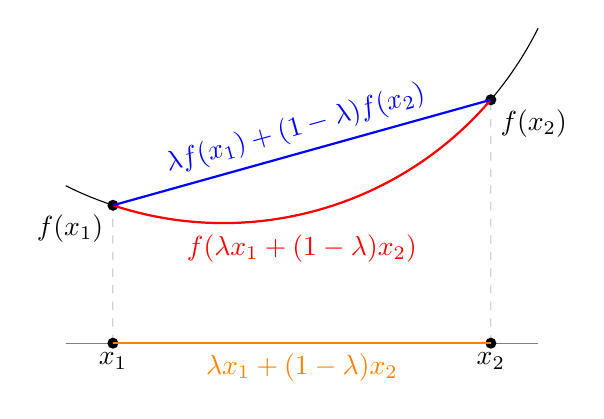
\begin{tikzpicture}[scale=2]
		\draw [name path=curve] (0,1) to [bend right=45] (3,2);
		\draw [help lines] (0,0) -- (3,0);
		\coordinate (x1) at (0.3,0);
		\coordinate (x2) at (2.7,0);
		\path [name path=vert1] (x1) -- ++(0,2);
		\path [name path=vert2] (x2) -- ++(0,2);
		\path [name intersections={of=curve and vert1, by=fx1}];
		\path [name intersections={of=curve and vert2, by=fx2}];
		\draw [help lines,dashed] (x1) -- (fx1);
		\draw [help lines,dashed] (x2) -- (fx2);
		\fill [black] 
			(x1)  circle (1pt) node [below] {$x_1$}
			(fx1) circle (1pt) node [below left] {$f(x_1)$}
			(x2)  circle (1pt) node [below] {$x_2$}
			(fx2) circle (1pt) node [below right] {$f(x_2)$};
		
		\onslide<2->{
			\draw [orange,thick] (x1) -- (x2) node [below, midway] {$\lambda x_1 + (1-\lambda)x_2$};
		}
		
		\onslide<3->{
			\begin{scope}
				\clip (x1) rectangle (fx2);
				\draw [red,thick] (0,1) to [bend right=45] (3,2);
			\end{scope}
			\node [red] at (1.5,0.6) {$f(\lambda x_1 + (1-\lambda)x_2)$};
		}
		
		\onslide<4->{
			\draw [blue,thick] (fx1) -- (fx2) node [above,midway,sloped] {$\lambda f(x_1) + (1-\lambda)f(x_2)$};
		}
	\end{tikzpicture}
\end{center}

\end{frame}

\begin{frame}{Convex functions with convex domains have only global minima.}

A function $f$ is convex if and only if
\[ {\color{red} f(\lambda\Vx_1 + (1-\lambda)\Vx_2)} \le {\color{blue} \lambda f(\Vx_1) + (1-\lambda)f(\Vx_2)}, \quad \lambda \in [0,1] \]

Here is a function with local minima. However, it isn't convex.

\begin{center}
	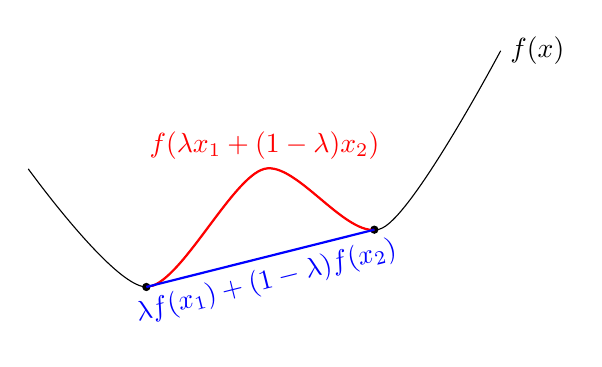
\begin{tikzpicture}[scale=1.5]
		\draw plot [smooth] coordinates {(0,0) (1,-1) (2,0) (3,-0.5) (4,1)} node [right] {$f(x)$};
		
		\coordinate (fx1) at (1,-1);
		\coordinate (fx2) at (2.93,-0.515);
		
		\fill (fx1) circle (1pt) (fx2) circle (1pt);
		
		\onslide<2->{
			\begin{scope}
				\clip (fx1) rectangle (2.93,1);
				\draw [red,thick] plot [smooth] coordinates {(0,0) (1,-1) (2,0) (3,-0.5) (4,1)};
			\end{scope}
			\node [red,above] at (2,0) {$f(\lambda x_1 + (1-\lambda)x_2)$};
		}
		
		\onslide<3->{
			\draw [blue,thick] (fx1) -- (fx2) node [below,midway,sloped] {$\lambda f(x_1) + (1-\lambda)f(x_2)$};
		}
	\end{tikzpicture}
\end{center}
	
\end{frame}

\begin{frame}{Why does the domain need to be convex?}

Imagine minimizing a convex function over a discontinuous (non-convex) domain (shaded blue).

\begin{center}
	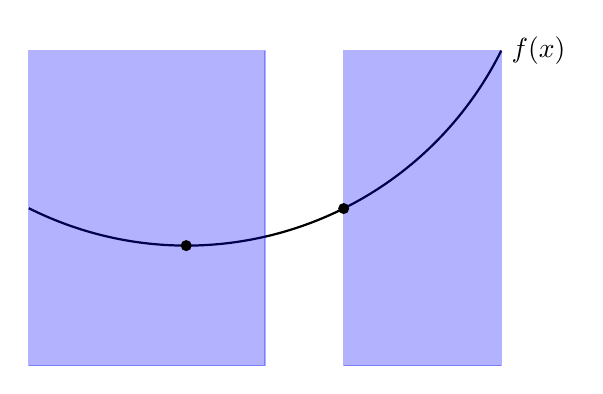
\begin{tikzpicture}[scale=2]
			\draw [name path=curve,thick] (0,1) to [bend right=45] (3,2) node [right] {$f(x)$};
			\coordinate (x1) at (1,0);
			\coordinate (x2) at (2,0);
			\path [name path=vert1] (x1) -- ++(0,2);
			\path [name path=vert2] (x2) -- ++(0,2);
			\path [name intersections={of=curve and vert1, by=fx1}];
			\path [name intersections={of=curve and vert2, by=fx2}];
			
			\filldraw [blue,opacity=0.3] (0,0) rectangle (1.5,2);
			\filldraw [blue,opacity=0.3] (2,0) rectangle (3,2);
			\onslide<2->{
				\fill [black] (fx1) circle (1pt);
				\fill [black] (fx2) circle (1pt);
			}
	\end{tikzpicture}
\end{center}

\onslide<2->{
	The boundaries create a second local (but not global) minimum of the convex function.
}
\end{frame}

\begin{frame}{The Jacobian Matrix}
Consider a multivariate function $\V{g}(\Vx) = \vecthree{g_1(\Vx)}{g_2(\Vx)}{g_3(\Vx)}$

\medskip
The Jacobian matrix of partial derivatives is
\[ \V{J}(\Vx) = \begin{pmatrix} 
	\dd{g_1}{x_1} & \dd{g_1}{x_2} & \dd{g_1}{x_3} \\ \\
 	\dd{g_2}{x_1} & \dd{g_2}{x_2} & \dd{g_2}{x_3} \\ \\
 	\dd{g_3}{x_1} & \dd{g_3}{x_2} & \dd{g_3}{x_3} \\
 \end{pmatrix} \]

\pause
\[ \V{g}(\Vx) = \vecthree{x_1x_2x_3}{x_2^2-x_1x_3}{2x_1^3} \quad \Rightarrow \quad \V{J}(\Vx) = \begin{pmatrix}
 	x_2x_3 & x_1x_3 & x_1x_2 \\
 	-x_3 & 2x_2 & -x_1 \\
 	6x_1^2 & 0 & 0	
 \end{pmatrix} \]

\end{frame}

\begin{frame}{The pseudoinverse}

Imagine a linear system $\VA\Vx = \Vy$. If \VA\ is square and full rank, then it has a true inverse $\VA^{-1}$. We can use the inverse to solve for $\Vx$:
\[ \Vx = \VA^{-1}\Vy \]

\pause
What if \VA\ is not square or not full rank? It still has a pseudoinverse $\VA^+$ that we can use to solve for \Vx:
\[ \Vx = \VA^+\Vy \]

\pause
If \VA\ is not full rank there are often infinitely many solutions to the linear system. Solving with the pseudoinverse gives the \emph{least squares} solution, i.e.\ the solution that minimizes the elementwise squared difference between $\VA\Vx$ and $\Vy$. The least squares solution is ideal for building linear models.

\pause
\bigskip
Final note: If the matrix $\transpose{\VA}\VA$ has full column rank, then $\VA^+ = (\transpose{\VA}\VA)^{-1}\transpose{\VA}$. Otherwise, we find the pseudoinverse using the Singular Value Decomposition (as we will see in Part~III).
\end{frame}

\begin{frame}{Interpreting the output of \texttt{fitlm}}

\begin{center}
	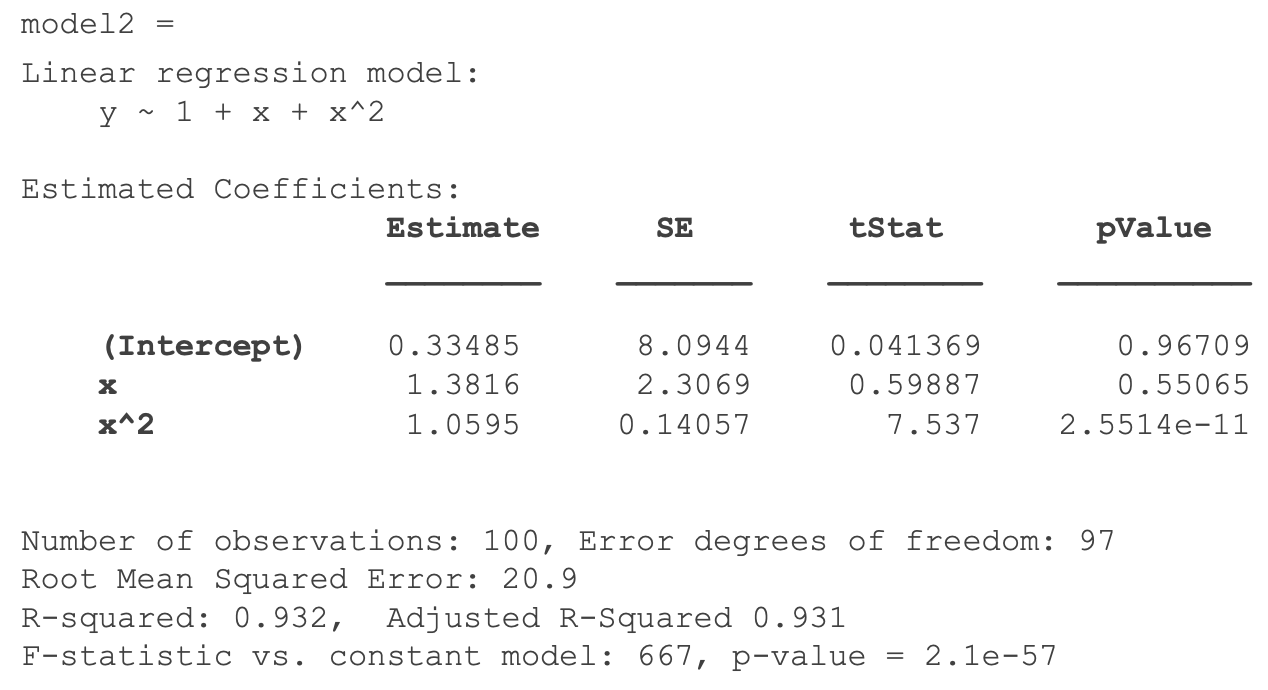
\includegraphics[width=0.8\textwidth]{fitlm-output}
\end{center}
{\small
\begin{itemize}
	\item \textbf{Estimate}: The estimated values of the parameter ($\beta_i$).
	\item \textbf{SE}: The standard error of the estimate. Roughly, if $\beta\pm 2$~SE includes 0, the parameter is not significant, but we prefer judgements based on the $p$-value of a $t$-test (below).
	\item \textbf{tStat}: The $t$-statistic used to calculate the $p$-value. Not directly interpretable.
	\item \textbf{pValue}: The probability that a nonzero parameter estimate of this size could have occurred randomly. If $p < 0.05$, we say the parameter is significantly nonzero.
\end{itemize}
}
\end{frame}

\begin{frame}{Why predict $\log(\mathrm{odds})$ in logistic regression?}

Remember that for logistic regression we use a linear model to predict the $\log(\mathrm{odds})$, i.e.\
\[ \log(\mathrm{odds}(y=1)) = \beta_0 + \beta_1x_1 + \cdots + \beta_nx_n \]

\pause
Why log odds? Two reasons:
\begin{itemize}
	\item The odds of an event is always non-negative, and we have no way of forcing our linear model to only make non-negative predictions. However, the log odds can take any value, with negative values indicating odds~$<1$.
	\item When we pass the log odds through the logistic link function, the output becomes the probability $P(y=1)$. This is easier to interpret and can be compared with binary data during model fitting.
\end{itemize}

\end{frame}

\begin{frame}{Deriving estimators}
\begin{enumerate}
	\item The goal of model fitting is to find parameters that minimize the \emph{loss}.
	\item For example, the quadratic loss for a model is
	\[ L(\boldsymbol{\beta}) = \sum_{i=1}^n\left( y_i^\text{pred}(\boldsymbol{\beta}) - y_i^\text{true} \right)^2 \]
	\pause
	\item We substitute the model in for $y^\text{pred}$ and minimize, usually by finding roots of the gradient with respect to $\boldsymbol{\beta}$. 
\end{enumerate}
\end{frame}

\begin{frame}{Newton's Method vs.\ Gradient descent}

\begin{columns}
\begin{column}{0.5\textwidth}
	We use Newton's method to find the roots of a multivariate function $\V{g}(\Vx)$.
	
	\begin{enumerate}
		\item Compute $\V{J}(\Vx)$, the Jacobian of $\V{g}$.
		\item Start with an initial guess $\Vx^{(0)}$.
		\item Iterate: \[ \Vx^{(1)} = \Vx^{(0)} - \V{J}^{-1}(\Vx^{(0)})\V{g}(\Vx^{(0)}). \]
		\item Repeat until \[ \V{g}(\Vx^{(k)}) \approx 0 \] or \[ \Vx^{(k)} \approx \Vx^{(k-1)}. \]
	\end{enumerate}
\end{column}
\begin{column}{0.5\textwidth}
	We use gradient descent to minimize a scalar-valued function $f(\Vx)$.
	
	\begin{enumerate}
		\item Comptute $\V{g}(\Vx)$, the gradient of $f$.
		\item Start with an initial guess $\Vx^{(0)}$.
		\item Iterate: \[ \Vx^{(1)} = \Vx^{(0)} - \alpha \V{g}(\Vx^{(0)}). \]
		\item Repeat until \[ f(\Vx^{(k)}) \approx f(\Vx^{(k-1)}) \] or \[ \Vx^{(k)} \approx \Vx^{(k-1)}. \]
	\end{enumerate}
\end{column}
\end{columns}

	
\end{frame}


\end{document}
